\section{Relação entre pontos e círculos}

\begin{frame}[fragile]{Relação de pertinência de um ponto $P$}

    \begin{itemize}
        \item Dado um ponto $P$ e um círculo de centro $C$ e raio $r$, uma (e apenas uma) das três 
            afirmações abaixo será verdadeira:

        \begin{enumerate}
            \item $P$ está dentro do círculo
            \item $P$ está sobre o círculo
            \item $P$ está fora do círculo
        \end{enumerate}

        \item Para determinar qual é a relação válida, basta computar a distância entre o ponto $P$
            e o centro $C$ do círculo

        \item Caso esta distância seja menor, igual ou maior que $r$, $P$ estará dentro, sobre e 
            fora do círculo, respectivamente

        \item O conjunto de pontos que estão dentro do círculo é denominado disco de raio $r$ e
            centro $C$
   \end{itemize}
\end{frame}

\begin{frame}[fragile]{Implementação da posição do ponto em um círculo em C++}
    \inputcode{cpp}{position.cpp}
\end{frame}

\begin{frame}[fragile]{Construção de círculos a partir de pontos}

    \begin{itemize}
        \item É possível identificar o(s) círculo(s) que interceptam um conjunto de $N$ pontos dados
    
        \item No caso $N = 1$, existem infinitos círculos (com infinitos raios possíveis) que 
            passam por um dado ponto $P$

        \item O caso $N = 2$ se torna mais interessante se o raio $r$ for pré-determinado

        \item Dados dois pontos $P$ e $Q$ e o um raio $r$, os cenários possíveis são:

        \begin{enumerate}
            \item $P = Q$: esta situação é idêntica ao caso $N = 1$
            \item $\mathrm{dist}(P, Q) = 2r$: se a distância entre os dois pontos dados é igual ao 
                diâmetro do círculo, existe um único círculo de raio $r$ que passa por $P$ e $Q$, 
                    cujo centro será o ponto médio do segmento $PQ$
            \item $\mathrm{dist}(P, Q) > 2r$: neste caso, nenhum círculo de $r$ pode passar por 
                ambos pontos simultaneamente
            \item $\mathrm{dist}(P, Q) < 2r$: neste caso, exatamente dois círculos passam por $P$ e $Q$ com raio $r$
        \end{enumerate}
    \end{itemize}

\end{frame}

\begin{frame}[fragile]{Implementação da identificação de um círculo a partir de dois pontos e o raio}
    \inputsnippet{cpp}{1}{20}{from_2_points.cpp}
\end{frame}

\begin{frame}[fragile]{Implementação da identificação de um círculo a partir de dois pontos e o raio}
    \inputsnippet{cpp}{21}{41}{from_2_points.cpp}
\end{frame}

\begin{frame}[fragile]{Demonstração do algoritmo}

    \begin{itemize}
        \item A implementação do algoritmo anterior, embora simples, é baseada em fatos não-triviais

        \item Sejam $P$ e $Q$ dois pontos distintos tais que $\mathrm{dist}(P, Q) < 2r$, onde
            $r$ é o raio dado

        \item Neste cenário, o centro $C$ do círculo não pertence ao segmento $PQ$

        \item Assim, é formado um triângulo $PCQ$

    \end{itemize}

    \begin{figure}
        \centering

        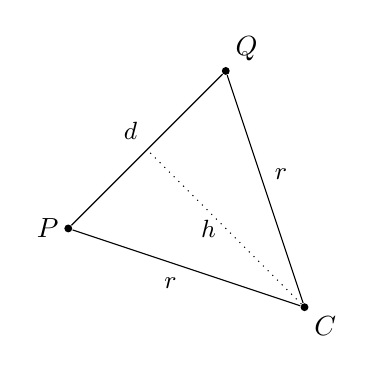
\begin{tikzpicture}
            \node[circle,inner sep=0pt,minimum size=1mm,fill] (P) at (1, 1) {};
            \node[circle,inner sep=0pt,minimum size=1mm,fill] (Q) at (3, 3) {};
            \node[circle,inner sep=0pt,minimum size=1mm,fill] (C) at (4, 0) {};
            \node[opacity=0,circle,inner sep=0pt,minimum size=1mm,fill] (R) at (2, 2) {};

            \draw (P) to node[midway,anchor=south east] { \small $d$ } (Q);
            \draw (P) to node[midway,anchor=north east] { \small $r$ } (C);
            \draw (Q) to node[midway,anchor=south west] { \small $r$ } (C);
            \draw[dotted] (C) to node[midway,anchor=east] { \small $h$ } (R);

            \node[anchor=east] at (P) { $P$ };
            \node[anchor=south west] at (Q) { $Q$ };
            \node[anchor=north west] at (C) { $C$ };

        \end{tikzpicture}
        
    \end{figure}

\end{frame}

\begin{frame}[fragile]{Demonstração do algoritmo}

    \begin{itemize}
        \item A Lei dos Cossenos diz que, num triângulo de lados $a, b, c$ cujo ângulo oposto
            a $a$ é $\alpha$, vale a igualdade
            \[
                a^2 = b^2 + c^2 - 2ab\cos \alpha
            \]

        \item Aplicando a Lei dos Cossenos ao triângulo $PCQ$, e considerando $\theta$
            o ângulo oposto ao lado $d$, têm-se que
        \[
            d^2 = r^2 + r^2 - 2r^2\cos \theta = 2r^2(1 - \cos \theta)
        \]

        \item Como $|\cos\theta| \leq 1$, vale a desigualdade
        \[
            d^2 \leq 4r^2,
        \]
        a qual pode ser reescrita como
        \[
            \frac{r^2}{d^2} \geq \frac{1}{4}
        \]
    \end{itemize}

\end{frame}

\begin{frame}[fragile]{Demonstração do algoritmo}

    \begin{itemize}
        \item Defina o discriminante
        \[
            \Delta = \frac{r^2}{d^2} - \frac{1}{4}
        \]

        \item Para que exista um círculo que passe por $P$ e $Q$ é preciso que $\Delta \geq 0$
    
        \item Como $PCQ$ é um triângulo isóceles, sua altura (cuma medida é $h$) coincide com a 
            mediana

        \item Seja $M$ o ponto médio de $PQ$. Aplicando o Teorema de Pitágoras ao triângulo $PMC$
            obtêm-se
        \[
            r^2 = h^2 + \left(\frac{d}{2}\right)^2, 
        \]
        isto é,
        \[
            h = \sqrt{r^2 - \frac{d^2}{4}} = d\sqrt{\frac{r^2}{d^2} - \frac{1}{4}} = d\sqrt{\Delta}
        \]
    \end{itemize}

\end{frame}

\begin{frame}[fragile]{Demonstração do algoritmo}

    \begin{itemize}
        \item Sejam $\vec{P}$ e $\vec{Q}$ os vetores-posição dos pontos $P$ e $Q$. O vetor 
            unitário $\vec{u}$ que parte de $P$ em direção a $Q$ é dado por
        \[
            \vec{u} = \frac{\vec{Q} - \vec{P}}{\| \vec{Q} - \vec{P}\|} = \left(\frac{x_Q - x_P}{d}, \frac{y_Q - y_P}{d}\right)
        \]

        \item O vetor unitário $\vec{n}$, normal a $\vec{u}$, é dado por
        \[
            \vec{n} = \left(\frac{y_P - y_Q}{d}, \frac{x_Q - x_P}{d}\right)
        \]

        \item Assim, o vetor posição do centro $C$ do círculo pode ser encontrado pela
            soma vetorial
        \[
            \vec{C} = \vec{P} + \frac{d}{2}\vec{u} + h\vec{n}
        \]

        \item As duas soluções possíveis diferem pelo sentido do vetor $\vec{n}$
    \end{itemize}

\end{frame}

\begin{frame}[fragile]{Demonstração do algoritmo}
    \begin{itemize}
        \item Portanto,
        \begin{align*}
            \vec{C} &= \vec{P} + \frac{d}{2}\vec{u} + h\vec{n} \\
            &= 
            \left(x_P, y_P\right) +
            \frac{d}{2}\left(\frac{x_Q - x_P}{d}, \frac{y_Q - y_P}{d}\right) + 
            h\left(\frac{y_P - y_Q}{d}, \frac{x_Q - x_P}{d}\right) \\
            &= 
            \left(x_P, y_P\right) +
            \left(\frac{x_Q - x_P}{2}, \frac{y_Q - y_P}{2}\right) + 
            d\sqrt{\Delta}\left(\frac{y_P - y_Q}{d}, \frac{x_Q - x_P}{d}\right) \\
            &= 
            \left(x_P, y_P\right) +
            \left(\frac{x_Q - x_P}{2}, \frac{y_Q - y_P}{2}\right) + 
            \sqrt{\Delta}\left({y_P - y_Q}, {x_Q - x_P}\right) \\
            &= 
            \left(\frac{x_P + x_Q}{2}, \frac{y_P + y_Q}{2}\right) + 
            \sqrt{\Delta}\left({y_P - y_Q}, {x_Q - x_P}\right) \\
        \end{align*}
    \end{itemize}

\end{frame}
